
%(BEGIN_QUESTION)
% Copyright 2009, Tony R. Kuphaldt, released under the Creative Commons Attribution License (v 1.0)
% This means you may do almost anything with this work of mine, so long as you give me proper credit

Draw connecting wires that will create a {\it parallel} circuit between all three resistors, such that current (conventional flow notation) will go through each resistor as shown by the arrows:

$$
\includegraphics[width=15.5cm]{i03807x01.eps}$$

\vskip 20pt \vbox{\hrule \hbox{\strut \vrule{} {\bf Suggestions for Socratic discussion} \vrule} \hrule}

\begin{itemize}
\item{} Supposing the battery has a voltage of 14 volts, and all resistors are 1 k$\Omega$ in resistance value, calculate the voltage dropped by each resistor.
\item{} Supposing the battery has a voltage of 14 volts, and all resistors are 1 k$\Omega$ in resistance value, calculate the current passing through each resistor as well as the current passing through the battery.
\end{itemize}

\underbar{file i03807}
%(END_QUESTION)





%(BEGIN_ANSWER)

$$\includegraphics[width=15.5cm]{i03807x02.eps}$$

%(END_ANSWER)





%(BEGIN_NOTES)

%INDEX% Pictorial circuit review (parallel resistor circuit)

%(END_NOTES)


